% ----------------------------------------------------------
\chapter{Project overview}
% ----------------------------------------------------------

% ----------------------------------------------------------
\section{VANT Architecture}
% ----------------------------------------------------------

ProVANT Emergencia is a \gls{UAV} prototype built in 70\% of it's designed size in Belo Horizonte, Brazil\footnotemark, comprised of a fuselage, which houses the electronic components, a V-Tail and wide wings with flaps, ailerons and wingtip nacelles, where the propeller lies. The propellers can rotate 180º to allow for a helicopter like flight and take-off, as can be seen in \autoref{fig:vant}. \cite{merchan_design_2021}

\footnotetext{A 100\% scale version is planned to be build in Universidad de Sevilla}

\begin{figure}[htb]
	\caption{\label{fig:vant}ProVANT Emergencia general mechanical structure view}
	\begin{center}
	    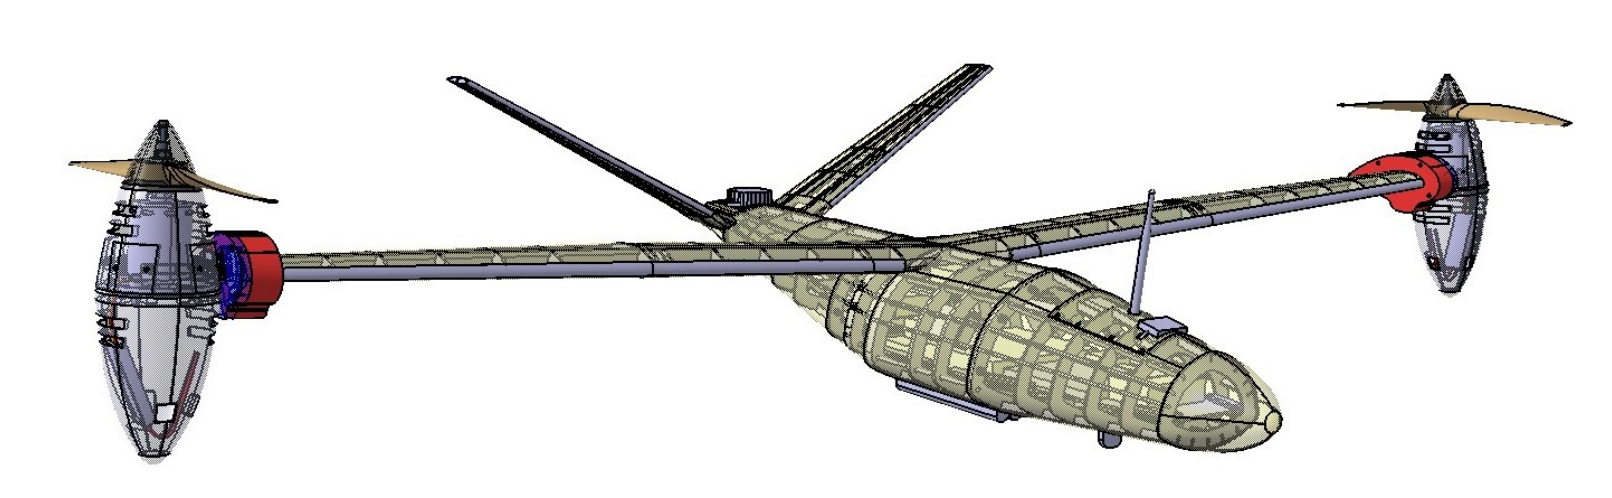
\includegraphics[width=.7\linewidth]{images/VANT.png}
	\end{center}
	\legend{Source: \textcite{merchan_design_2021}.}
\end{figure}

The embedded electronics, as described both by \textcite{lara_design_2019} and \textcite{merchan_design_2021} is developed around two types of embedded processors, called Low Level Hardware (\gls{LLH}) and High Level Hardware (\gls{HLH}). The \gls{LLH} is responsible for directly interfacing with the actuators and simple sensors. It is implemented by two redundant \href{https://www.st.com/en/evaluation-tools/nucleo-f767zi.html}{STM32 Nucleo-F767zi}. 
% Above a referenced the R2U2 site as a citation, here the ST site just by a link, which approach should I used

\begin{figure}[htb]
	\caption{\label{fig:nucleo}ProVANT Emergencia \gls{LLH} board (Nucleo-F767zi)}
	\begin{center}
	    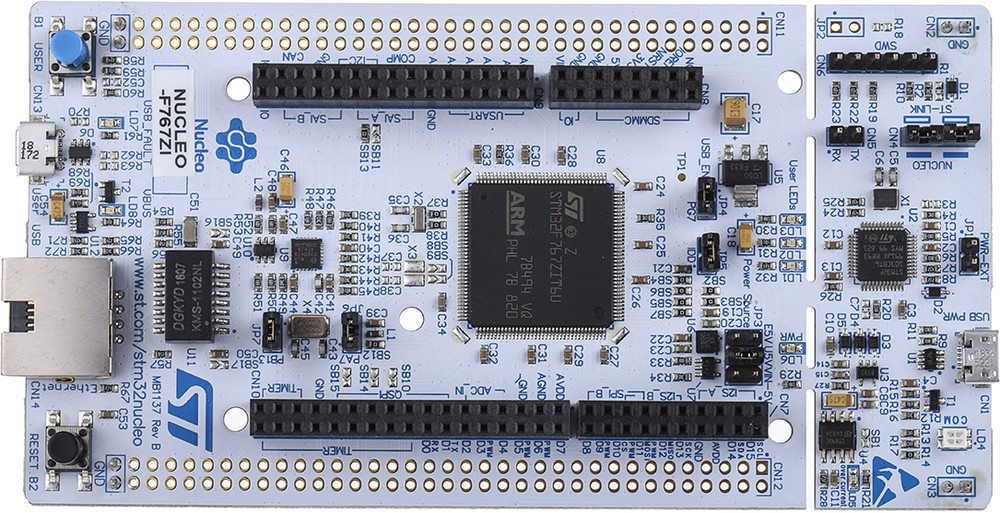
\includegraphics[width=.7\linewidth]{images/nucleo-f767zi.jpg}
	\end{center}
	\legend{Source: From an %russian marketplace 
    advertisement in \href{https://www.chipdip.ru/product/nucleo-f767zi-2}{Chipdip}} % Not great references, but ST website has only low quality images of the board
\end{figure}

The importance of having redundancy in these boards is that they are the only boards in the system with access to the actuators, therefore, in case of a failure in them the system would be incapable of controlling it self.
% if only one board ware used. 
With two Low Level boards, the chances of both failing is much smaller.
% both need to fail to make the system lose access to the actuators, which is a less likely scenario. % more unlikely scenario.

The main \gls{HLH} ti the Jetson Tx2 board, aimed to run the main control loop and chosen by the capability of running neural network, because of it's \gls{GPU} that allows for parallelization of the computing operations. It also interfaces with precise sensors with low latency reading requirements, like the IMU and GPS. \cite{lara_design_2019,merchan_design_2021}

\begin{figure}[htb]
	\caption{\label{fig:jetson}ProVANT Emergencia main \gls{HLH} board (Jetson Tx2)}
	\begin{center}
	    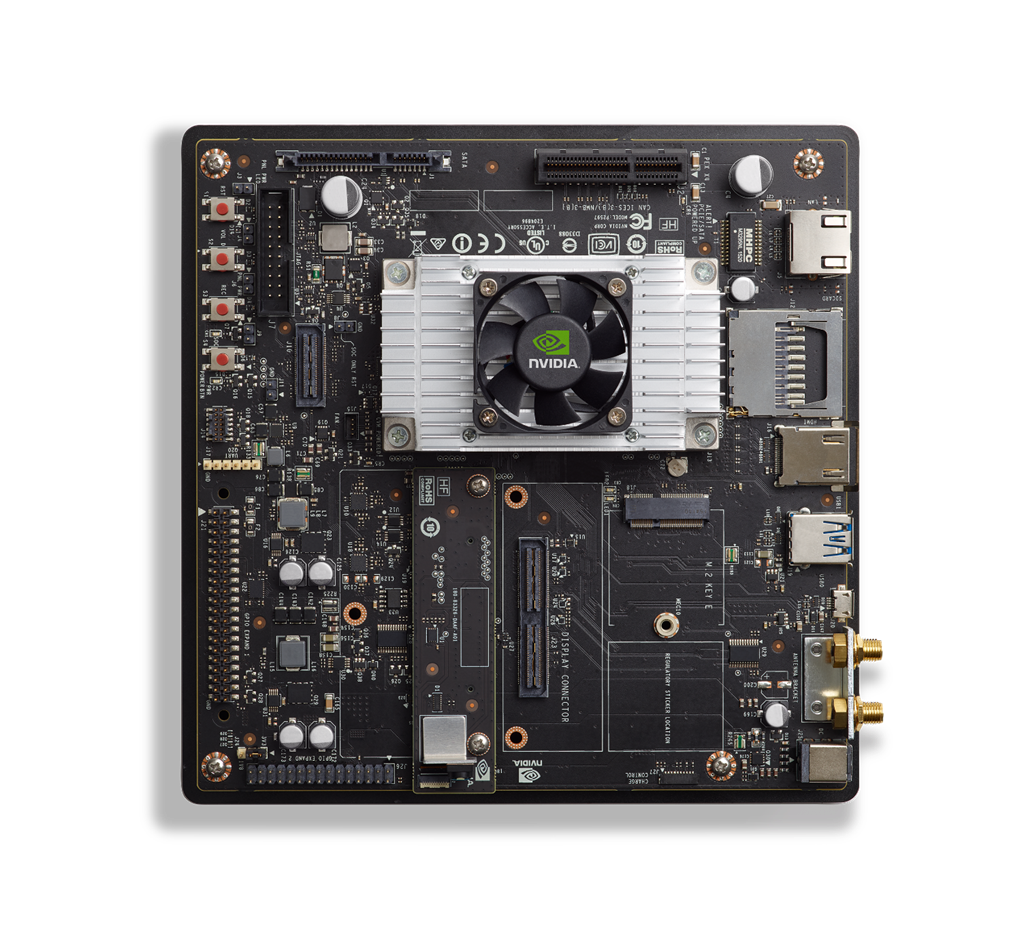
\includegraphics[width=.7\linewidth,trim=2.5cm 2cm 2.5cm 2cm]{images/JTX2_Devkit.png}
	\end{center}
	\legend{Source: From \href{https://www.google.com/url?sa=i\&url=https\%3A\%2F\%2Fdeveloper.nvidia.com\%2Fblog\%2Fjetson-tx2-delivers-twice-intelligence-edge\%2F&psig=AOvVaw1CFt5TyMwmZPdZhERPTBZo\&ust=1727813766519000\&source=images\&cd=vfe\&opi=89978449\&ved=0CBQQjRxqFwoTCMic8oG-64gDFQAAAAAdAAAAABAJ}{Nvidia's website}} 
\end{figure}

Since both aforementioned thesis, a new board was added along the Jetson in the High Level system to interface with the Navio 2 board and a telemetry radio. This board is a Raspberry Pi 4, it facilitates the communication with the Navio 2 board, which implements multiple useful sensors for drones and can generate \gls{PWM} for controlling of actuators. Navio 2 is made to be used with a Raspberry Pi, so using it was the easiest solution.

\begin{figure}[htb]
	\caption{\label{fig:raspberry}ProVANT Emergencia \gls{HLH} auxiliary board (Raspberry Pi 4)}
	\begin{center}
	    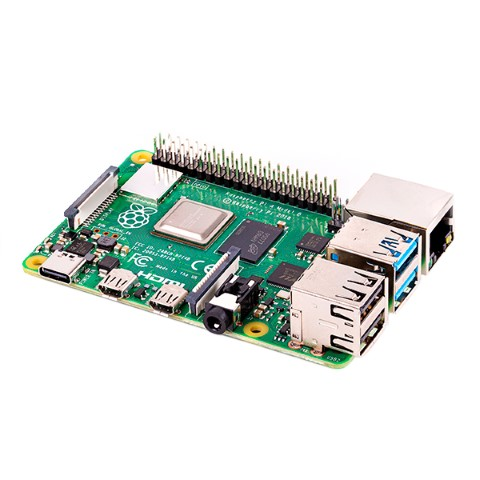
\includegraphics[width=.7\linewidth,trim=.8cm 4cm .8cm 4.3cm,clip]{images/raspberry.png}
	\end{center}
	\legend{Source: From \href{https://www.raspberrypi.com/products/raspberry-pi-4-model-b/}{Raspberry Pi's website}}
\end{figure}

Both Nucleos, the Jetson and Raspberry Pi are connected together in a communication network that implements standards internet protocols, with \gls{UDP} transport layer protocol instead of \gls{TCP}, for it's performance; and Ethernet as physical and link layer protocols. To avoid the non-deterministic characteristics of the standard \gls{CSMA/CD} medium access control protocol, a token ring protocol\footnotemark\ is implemented to avoid collisions.%\cite{noauthor_software_2024} % Não sei se eu posso citar, acho que nunca foi, e talvez nunca será publicado

\footnotetext{This means that only one of the machines will have the permission to use the network hardware. It's said that this board has the "token", and once the permission is given to other board, that the "token was handed" to the other computer.}

\begin{figure}[htb]
	\caption{\label{fig:elecHard}ProVANT Emergencia general electrical structure view}
	\begin{center}
	    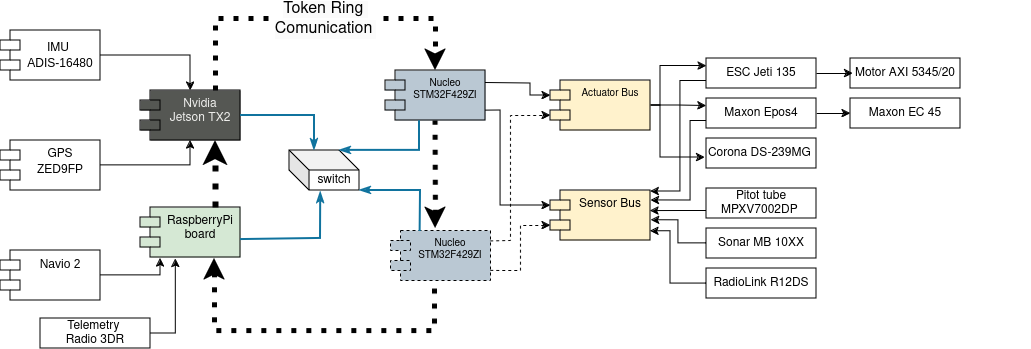
\includegraphics[width=\linewidth,trim=0cm 0cm 2.5cm 0cm,clip]{images/Hardware Setup.png}
	\end{center}
	\legend{Source: 
        %\textcite{noauthor_software_2024}}
        Personal archive} % É do projeto, acho que eu posso por como "pessoal"
\end{figure}


% ----------------------------------------------------------
\section{Fault models for ProVANT}
% ----------------------------------------------------------

When started up, Jetson controls the \gls{UAV} and the primary Nucleo controls the actuators according to the data received from the Jetson. The primary Nucleo should take control if the Jetson enters into a faulty state, likewise the secondary Nucleo has to get the control if both the Jetson and the primary Nucleo fails.

The state of liveliness of each board could be modeled as the \autoref{fig:liveliness}. The composition of this automata for each of the modules is equivalent of the state diagram proposed by \textcite{benica_design_2024} and shown in \autoref{fig:liveliness_full}, where colors are assigned to represent the severeness of the situation.

\begin{figure}[!htb]
    \centering
    \caption{\label{fig:liveliness} Per module liveliness status automata}
    \begin{tikzpicture}[->, >=Stealth, shorten >=1pt, auto, node distance=3cm, semithick]

  \node[state, initial] (q1) {alive};
  \node[state] (q2) [right of=q1] {dead};

  \path (q1) %edge [loop above] node {a} (q1)
            edge [bend left] node {fault} (q2)
        (q2) %edge [loop above] node {c} (q2)
            edge [bend left] node {recovered} (q1);

\end{tikzpicture}
    \legend{Source: Own elaboration}
\end{figure}

\begin{figure}[!htb]
    \centering
    \caption{\label{fig:liveliness_full} Full system liveliness status automata}
    \includegraphics[width=\linewidth,trim=3.2cm 17cm 2.7cm 3cm,clip]{images/Monografia___Daniel_Benicá_liveliness_estate_machine.pdf}
    \legend{Source: \textcite{benica_design_2024}}
\end{figure}

These status should be monitored by each of the modules in order to verify the safeties requirements
and for the correct operation of the token ring protocol, as the tokens shouldn't be given to an unresponsive board. % Need to verify how the token gets transmitted
A possible implementation could be adding a flag at the Module class, or \textit{struct} in case of the c code used in the Nucleos.

To do so, it is necessary to implement techniques to identify faulty boards in the system. As boards should continuously monitor their own behavior with \gls{RV}, it could be the case that a faulty board inform the others about it's faults prior to trying to recover, for example by a reset. However this scenario cannot be considered always possible, unforeseen faults may cause the board to reset or shutdown without warning, or even be unable to communicate.

\textcite{benica_design_2024} proposes methods to identify faults in the system. These methods being: heartbeat, watchdog, network monitoring and exception notification. Heartbeat means periodic messages, called heartbeats, sent by each of the boards inform the normal behavior, missing heartbeats inform a disconnection, this can help to identify a fault on a board that couldn't have communicated it. The watchdog is a timer that needs to be periodically reset by code, allowing the watchdog to overflow could mean the code is not executing or is in a deadlock. Network monitoring is simply calculating the latency of the network and the occurrence of missing messages. Exceptions notification is the common implementation of exceptions in code which can be catch by a catch statement and dealt with in code, one of the proposed ways of dealing with exception was the communication through the network.

\textcite{benica_design_2024} also proposes that the state of each of the boards should follow the \autoref{fig:banica_state}, where the 
\begin{tikzpicture}[auto, semithick]
\node[draw=black, fill=red, circle, inner sep=0.5mm] {\scriptsize\textcolor{black}{\textbf{x}}};
\end{tikzpicture} symbol represents the possibility of occurring a fault in that state, which triggers a transition to the state marked with 
\begin{tikzpicture}[auto, semithick]
\node[draw=black, fill=red, circle, inner sep=0.5mm] {\scriptsize\textcolor{red}{\textbf{x}}};
\end{tikzpicture}.

\begin{figure}[!htb]
    \centering
    \caption{\label{fig:banica_state} State machine for each board}
    \begin{tikzpicture}[->, >=Stealth, shorten >=1pt, auto, node distance=3cm, semithick]

    % \node[state, initial] (q1) {Unconfigured};
    % \node[state] (init) [below of=q1] {Initializing};
    % \node[state] (pre) [below of=init] {Pre-flight};
    % \node[state] (auto) [below of=pre, yshift=-.5cm] {Autonomous};
    % \node[state] (standby) [left of=auto] {Standby};
    % \node[state] (man) [right of=auto] {Manual};
    % \node[state] (shut) [below of=auto, yshift=-.5cm] {Shutdown};
    % \node[state] (diag) [right of=pre, xshift=2cm] {Diagnostics};
    % \node[state] (recov) [left of=init, xshift=-3cm] {Recovery};

    \node[state, initial, rectangle, rounded corners] (q1) {Unconfigured};
    \node[state, rectangle, rounded corners] (init) [below of=q1] {Initializing};
    \node[state, rectangle, rounded corners] (pre) [below of=init] {Pre-flight};
    \node[state, rectangle, rounded corners] (auto) [below of=pre, yshift=-.5cm] {Autonomous};
    \node[state, rectangle, rounded corners] (standby) [left of=auto] {Standby};
    \node[state, rectangle, rounded corners] (man) [right of=auto] {Manual};
    \node[state, rectangle, rounded corners] (shut) [below of=auto, yshift=-.5cm] {Shutdown};
    \node[state, rectangle, rounded corners] (diag) [right of=pre, xshift=2cm] {Diagnostics};
    \node[state, rectangle, rounded corners] (recov) [left of=init, xshift=-3cm] {Recovery};

  \path (q1) %edge [loop above] node {a} (q1)
            edge node {} (init)
        (init) %edge [loop above] node {c} (q2)
            edge node {} (pre)
        (pre)
            edge [bend right=10] node {} (standby)
        (pre)
            edge node {} (auto)
        (pre)
            edge [bend left=10] node {} (man)
        (standby)
            edge [bend left] node {} (auto)
        (auto)
            edge [bend left] node {} (standby)
        (man)
            edge [bend left] node {} (auto)
        (auto)
            edge [bend left] node {} (man)
        (standby)
            edge [bend left=50] node {} (man)
        (man)
            edge [bend left=50] node {} (standby)
        (auto)
            edge node {} (shut)
        (standby)
            edge [bend right=10] node {} (shut)
        (man)
            edge [bend left=10] node {} (shut);

        \path (pre)
            edge [bend left] node {} (diag)
        (diag)
            edge [bend left] node {} (pre);

        \path (recov)
            edge node [above, yshift=.25cm]{Not in flight} (pre)
        (recov)
            edge node [left]{In flight} (standby);
    
    % \node[draw=black, fill=red, circle, inner sep=0.5mm] at ([xshift=0.88cm, yshift=0.55cm]init) {\textcolor{black}{\textbf{x}}};
    % \node[draw=black, fill=red, circle, inner sep=0.5mm] at ([xshift=0.8cm, yshift=0.5cm]pre) {\textcolor{black}{\textbf{x}}};
    % \node[draw=black, fill=red, circle, inner sep=0.5mm] at ([xshift=1.04797cm, yshift=0.757cm]auto) {\textcolor{black}{\textbf{x}}};
    % \node[draw=black, fill=red, circle, inner sep=0.5mm] at ([xshift=0.72cm, yshift=0.45cm]man) {\textcolor{black}{\textbf{x}}};
    % \node[draw=black, fill=red, circle, inner sep=0.5mm] at ([xshift=0.88cm, yshift=0.55cm]shut) {\textcolor{black}{\textbf{x}}};
    % \node[draw=black, fill=red, circle, inner sep=0.5mm] at ([xshift=0.88cm, yshift=0.55cm]recov) {\textcolor{red}{\textbf{x}}};

    \node[draw=black, fill=red, circle, inner sep=0.5mm] at ([xshift=0.88cm, yshift=0.55cm]init) {\textcolor{black}{\textbf{x}}};
    \node[draw=black, fill=red, circle, inner sep=0.5mm] at ([xshift=0.8cm, yshift=0.55cm]pre) {\textcolor{black}{\textbf{x}}};
    \node[draw=black, fill=red, circle, inner sep=0.5mm] at ([xshift=1.04797cm, yshift=0.55cm]auto) {\textcolor{black}{\textbf{x}}};
    \node[draw=black, fill=red, circle, inner sep=0.5mm] at ([xshift=0.72cm, yshift=0.55cm]man) {\textcolor{black}{\textbf{x}}};
    \node[draw=black, fill=red, circle, inner sep=0.5mm] at ([xshift=0.88cm, yshift=0.55cm]shut) {\textcolor{black}{\textbf{x}}};
    \node[draw=black, fill=red, circle, inner sep=0.5mm] at ([xshift=0.88cm, yshift=0.55cm]recov) {\textcolor{red}{\textbf{x}}};
\end{tikzpicture}
    \legend{Source: \textcite{benica_design_2024} (revised)}
\end{figure}

Problems may arise while integrating the heartbeat technique 
% described by \textcite{benica_design_2024} 
with the token ring protocol, as the designer has decide weither the heartbeat messages should ignore the token, and only data messages have to be send when the board possesses the token, or it should respect the protocol.


% \textbf{Instruções da Coordenação do PFC:}

% Neste capítulo, deve-se apresentar (de forma mais detalhada e aprofundada tecnicamente que na Introdução):
% \begin{itemize}
% 	\item O contexto e a motivação do PFC;
% 	\item Descrição da empresa/instituto de pesquisa (histórico, clientes, produtos, serviços, projetos, etc) em que o PFC foi realizado e do projeto global da empresa em que o PFC está inserido (se for o caso);
%      \item Descrição do problema tratado no PFC;
%      \item Requisitos técnicos (funcionais e não-funcionais).
% \end{itemize}

% Procure utilizar equações, tabelas, diagramas e fluxogramas para ilustrar e explicar melhor as ideias.
